\documentclass{article}

\usepackage[utf8]{inputenc}
\usepackage{subcaption}
\usepackage{caption}
\usepackage{amssymb}
\usepackage{amsmath}
\usepackage[a4paper,total={7in, 8in}]{geometry}
% \usepackage[hidelinks]{hyperref} % Commented out to avoid option clash
\usepackage{bm}
\usepackage{centernot}
\usepackage{titling}
\usepackage{color}
\usepackage{listings}
\usepackage{graphicx} % Required for inserting images
\usepackage{tikz}
\tikzstyle{mybox} = [draw=black, thin, rectangle, rounded corners, inner ysep=5pt, inner xsep=5pt, fill=orange!20]


%Per disegnare il box
%\hspace*{-5mm}
%\begin{tikzpicture}
%\node [mybox] (box){%
%    \begin{minipage}{.96\textwidth}     %Larghezza del box
            %Qui testo
%    \end{minipage}
%};
%\end{tikzpicture}%



\title{\textbf{[Manuale di Sviluppo] Realizzazione di un ambiente di Fault Injection
per applicazione ridondata }}
\author{Carlo Migliaccio (s332937) - Federico Pretini (s) -\\
Scavone Alessandro (s328782) -  Mattia Viglino (s)}
\date{Gennaio 2024}

\begin{document}
\counterwithin{figure}{section}
\counterwithin{equation}{section}
\renewcommand{\labelenumii}{\arabic{enumi}.\arabic{enumii}}

\maketitle

\tableofcontents

\section{Introduzione}
Nella società attuale si fa, in generale, un utilizzo capillare di sistemi computerizzati, questi nello specifico sono coinvolti in settori in cui un guasto al sistema potrebbe essere critico, mettendo potenzialmente a rischio vite umane. L'implementazione di sistemi \textit{safety-critical} espone lo sviluppatore ad affrontare problemi non trascurabili che coinvolgono la valutazione della \textbf{dependability} \cite{noauthor_dependability_2024} e della \textbf{tolleranza ai guasti} (\textit{fault tolerance}). Le tecniche di test standard e l'utilizzo di benchmark non bastano in quest'ambito, in quanto per valutare certi aspetti del sistema (quali la dependability) bisognerebbe osservarne il comportamento dopo che il guasto si verifica. \\
In ambito 'fault-tolerance' vengono utilizzate delle metriche specifiche per quantificare affidabilità e robustezza del sistema in analisi. Per citarne una significativa, riportiamo l'\textit{MTBF} (Mean Time Between Failure); questa per i sistemi concepiti, per essere tolleranti ai guasti, potrebbe essere associata ad un periodo di tempo molto lungo, anche anni! Da tempo la ricerca va nella direzione di trovare un modo per 'accelerare' in simulazione l'occorrenza di questi guasti/difetti prima che accadano naturalmente, dal momento che questa lunga latenza rende difficile anche solo identificare la causa di un potenziale difetto/guasto. In molti casi l'approccio utilizzato è quello basato su esperimenti di \textbf{fault injection}, che -- come riportato in \cite{depend} -- vengono usati non solo durante l'implementazione, ma anche durante la fase prototipale e operativa, permettendo quindi di coprire un ampio spettro di casistiche.\\
La survey \cite{hsueh1997fault} individua principalmente due grandi famiglie di \textit{tecniche di fault injection}:
(i) \textsc{Fault Injection Hardware} di cui non ci occupiamo; (ii) \textsc{Fault Injection Software}, è la famgilia  di tecniche che negli ultimi anni ha attirato l'interesse dei ricercatori in quanto tali metodi non richiedono hardware costoso. Inoltre nei contesti in cui il target sia un \textit{applicativo} o, ancora peggio, il \textit{sistema operativo}, costituiscono l'unica scelta.

\noindent
Nel lavoro qui presentato si adotta un approccio \textit{software} che si pone principalmente \textbf{due obiettivi}: 
\begin{enumerate}
    \itemsep-0.3em
    \item La modifica del codice per \textit{casi di studio scelti} volta ad introdurre ridondanza nel sistema tramite la \textbf{duplicazione di tutte le variabili}; 
    \item La realizzazione di un \textbf{ambiente software di fault injection} per simulare l'occorrenza di guasti nel sistema irrobustito e valutarne l'\textit{affidabilità}. Il \textbf{modello di fault} analizzato è il \textit{transient single bit-flip fault}, su cui si basano molti tool di fault injection. 
\end{enumerate}

\noindent 
Il presente documento si pone l'obiettivo di evidenziare i passaggi salienti dell'implementazione delle tecniche di \textit{Software fault tolerance} e dell'\textit{ambiente di fault injection} riportando schemi e \textit{code snippet}  che insieme al codice sorgente -- in \textbf{linguaggio Rust} -- permettono di seguire le diverse fasi del lavoro svolto.\\
Nella \textbf{Sezioni \ref{sec:hardened}-\ref{sec:transf_impl}} viene introdotto e successivamente implementato un \textbf{set di trasformazioni del codice} sfruttando parte dei concetti presentati in \cite{rebaudengo1999soft}. Si anticipa che l'implementazione di queste regole è integrata nella realizzazione di un nuovo tipo generico(\texttt{Hardened<T>}) di cui si descrivono gli aspetti chiave. La \textbf{Sezione \ref{sec:CaseStudies}} fornisce un'analisi comparativa del codice non irrobustito rispetto a quello che utilizza le variabili di tipo generico \texttt{Hardened<T>}. Nella \textbf{Sezione \ref{sec:Fault_Env}} viene definita la struttura dell'ambiente di fault injection, mentre le \textbf{Sezioni \ref{sec:FLM}, \ref{sec: Injector}, \ref{sec:analizer}} si occupano di analizzarne i componenti. Infine la \textbf{Sezione \ref{sec:Struttura_Codice}} descrive brevemente la struttura del codice sorgente e dei test d'unità.

\section{Software fault-tolerance} \label{sec:hardened}
In generale le tecniche di software fault-tolerance, tendono a sfruttare modifiche di alto livello al codice sorgente in modo da poter rilevare comportamenti irregolari (faults) che riguardano \textbf{sia il codice che i dati}. Qui invece \textit{poniamo l’attenzione esclusivamente su fault che riguardano i dati},  senza peraltro preoccuparci del fatto che questi si trovino in memoria centrale, memoria cache, registri o bus. Al codice target infatti vengono applicate semplici trasformazioni di alto livello che sono completamente indipendenti dal processore che esegue il programma. 
\subsection{Tre regole per la trasformazione del codice}
Le regole di trasformazione del codice citate sono quelle proposte in \cite{802887}. Riportiamo qui quelle mirate al rilevamento di \textbf{errori sui dati}:
\begin{enumerate}
    \itemsep-0.2em
    \item \textbf{Regola \#1}: Ogni variabile \texttt{x} deve essere duplicata: siano \texttt{cp1} e \texttt{cp2} i nomi delle due copie;
    \item \textbf{Regola \#2}: Ogni operazione di scrittura su \texttt{x} deve essere eseguita su entrambe le copie \texttt{cp1} e \texttt{cp2};
    \item \textbf{Regola \#3}:  dopo ogni operazione di lettura su $x$, deve essere controllata la consistenza delle copie \texttt{cp1} e \texttt{cp2}, nel caso in cui tale controllo fallisca deve essere sollevato un errore.
\end{enumerate}
Anche i parametri passati a una procedura, così come i valori di ritorno, sono variabili come tutte le altre a cui si applicano le stesse trasformazioni. L'implementazione di queste caratteristiche -- come spiegato in dettaglio nel paragrafo successivo -- si basano sulla programmazione generica e polimorfismo offerti dal linguaggio Rust. Dopo una prima analisi si descrivono le principali caratteristiche e i metodi offerti dal nuovo tipo, in un secondo momento si entra nel dettaglio del linguaggio e si pone l'attenzione all'implementazione della semantica richiesta da \textbf{(R1)-(R3)}.

\subsection{Il tipo \texttt{Hardened<T>}}
Le tre regole di trasformazione appena esposte sono espletate tramite l'implementazione di un \textbf{nuovo tipo}, che chiamiamo \texttt{Hardened<T>}, definito come segue: 

\begin{lstlisting}[language=Rust, style=boxed]
#[derive(Clone, Copy)]
struct Hardened<T>{
    cp1: T, 
    cp2: T
}
\end{lstlisting}
\noindent
Poiché si vuole porre l'attenzione sul comportamento/algoritmo di questo nuovo tipo, si usa la programmazione generica infatti le due copie \texttt{cp1} e \texttt{cp2} hanno un tipo generico \texttt{T} a cui viene posto l'unico vincolo di essere confrontabile e copiabile.
Con l'obiettivo di coprire il maggior numero di casistiche possibili in cui il dato viene acceduto in lettura e/o scrittura, sono stati implementati per \texttt{Hardened<T>} un numero significativo di \textbf{tratti della libreria standard}, in particolare: 
\begin{itemize}
    \itemsep-0.3em
    \item \texttt{From<T>}: per ricavare una variabile ridondata a partire da una variabile 'semplice' di tipo T; 
    \item I tratti per le \textbf{operazioni aritmetiche} \texttt{Add, Sub, Mul}. In particolare i primi sono stati implementati anche in \textit{versione mista} \texttt{Add<usize>} e \texttt{Sub<usize>} per semplificare le operazioni di sottrazione tra un \texttt{Hardened<T>} e un valore \textit{literal}; 
    \item I tratti per le \textbf{operazioni di confronto} \texttt{Eq, PartialEq, Ord, PartialOrd}; 
    \item I tratti \texttt{Index} e \texttt{IndexMut} sotto diverse forme per accedere alla singola copia della variabile (utile in fase di iniezione) e all'elemento i-esimo di una \textit{collezione} di \texttt{Hardened<T>}.
    \item Il tratto \texttt{Debug} per la visualizzazione personalizzata di informazioni sul nuovo tipo di dato.
\end{itemize}

\noindent
Oltre ai tratti della libreria standard appena elencati,  si è rivelata utile l'implementazione di funzioni personalizzate di cui si riporta una breve descrizione.
\begin{lstlisting}[language=Rust, style=boxed]
impl<T> Hardened<T>{
    fn incoherent(&self)->bool;
    pub fn assign(&mut self, other: Hardened<T>)->Result<(), IncoherenceError>;
    pub fn from_vec(vet: Vec<T>)->Vec<Hardened<T>>;
    pub fn from_mat(mat: Vec<Vec<T>>) -> Vec<Vec<Hardened<T>>>;
    pub fn inner(&self)->Result<T, IncoherenceError>;
}
\end{lstlisting}

\begin{description}
    \item[\texttt{fn incoherent(\&self)->bool}] Funzione privata per rilevare l'incoerenza tra le due copie della variabile irrobustita: in particolare viene utilizzata dai metodi di più alto livello che lavorano con i dati elementari.
    \item[\texttt{pub fn assign(\&mut self, other: Hardened<T>)->Result<(), IncoherenceError>;}]\quad \newline Asserisce all'\textbf{assegnazione} tra due variabili di tipo \texttt{Hardened<T>}. Questa è l'unica operazione che non si può ridefinire in Rust tramite l'implementazione del tratto opportuno, in quanto andrebbe ridefinita l'intera semantica legata al \textbf{movimento e possesso}.
    \item[\texttt{ pub fn from\_vec(vet: Vec<T>)->Vec<Hardened<T>>;} ] Per estrarre collezioni di dati irrobustiti da collezioni di dati elementari. Un ruolo simile è svolto da \newline \texttt{pub fn from\_mat(mat: Vec<Vec<T>>) -> Vec<Vec<Hardened<T>>>;} Queste funzioni sono indispensabili sia per l'implementazione che per l'analisi dei risultati dei casi di studio.
    \item[\texttt{pub fn inner(\&self)->Result<T, IncoherenceError>;}] esegue una sorta di \textit{unwrap} del dato irrobustito, cioè dato un \texttt{Hardened<T>} restituisce il dato \texttt{T} incapsulato a sua volta in un \texttt{Result} in quanto le copie memorizzate possono essere incoerenti (vedi paragrafo dopo).
\end{description}

\section{Regole di trasformazione: implementazione}\label{sec:transf_impl}
In questo paragrafo, tramite l'utilizzo di esempi significativi si presenta a grandi linee l'implementazione del set di trasformazioni che portano al tipo irrobustito. In particolare, dopo aver richiamato la regola, segue un esempio di codice con l'implementazione.\\

\noindent
\begin{center}
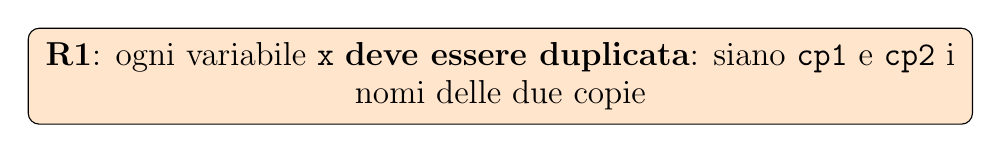
\begin{tikzpicture}
    \node [mybox] (box){%
        \begin{minipage}{.96\textwidth}    
                \begin{center}
                    \large
                \textbf{R1}: ogni variabile \texttt{x} \textbf {deve essere duplicata}: siano \texttt{cp1} e \texttt{cp2} i nomi delle due copie
                \end{center}
        \end{minipage}
    };
\end{tikzpicture}%
\end{center}

\noindent
La realizzazione della prima regola è insita nella definizione del nuovo tipo, in quanto una dichiarazione l'inizializzazione di una variabile a partire da un dato elementare, crea una doppia copia del dato stesso. Si veda il seguente esempio: 
\begin{lstlisting}[language=rust, style=boxed]
let mut myvar=15; 
let mut hard_myvar = Hardened::from(myvar);
\end{lstlisting}
Tramite il metodo \texttt{from()} del tratto \texttt{From} infatti vengono popolati i campi \texttt{cp1} e \texttt{cp2} della nuova variabile \texttt{hard\_myvar} nel modo seguente: 

\begin{lstlisting}[language=rust, style=boxed]
impl<T> From<T> for Hardened<T> where T:Copy{
    fn from(value: T) -> Self {
        // Regola 1: duplicazione delle variabili
        Self{cp1: value, cp2: value}
    }
}   
\end{lstlisting}

\noindent
\begin{center}
    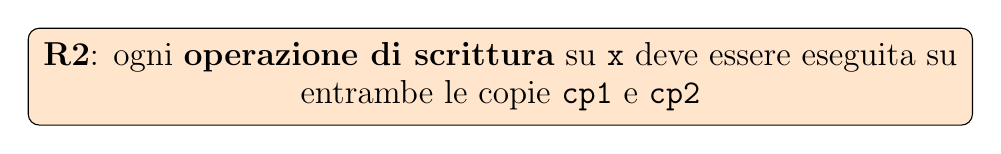
\begin{tikzpicture}
        \node [mybox] (box){%
            \begin{minipage}{.96\textwidth}    
                \begin{center}
                    \large
                    \textbf{R2}: ogni \textbf{operazione di scrittura} su \texttt{x} deve essere eseguita su entrambe le copie \texttt{cp1} e \texttt{cp2}
                \end{center}
            \end{minipage}
        };
    \end{tikzpicture}%
\end{center}
Come esempio significativo si consideri il frammento di codice dell'operazione di \texttt{assign()}:

\begin{lstlisting}[language=rust, style=boxed]
pub fn assign(&mut self, other: Hardened<T>)->Result<(), IncoherenceError>{
    //                  [... ]

    //Regola 2: Ogni scrittura deve essere eseguita su entrambe le copie
    self.cp1 = other.cp1;
    self.cp2 = other.cp2;
    Ok(())
}
\end{lstlisting}
Dopo un controllo di coerenza della variabile da assegnare (paragrafo successivo), si scrive sia su una copia che sull'altra.

\noindent
\begin{center}
    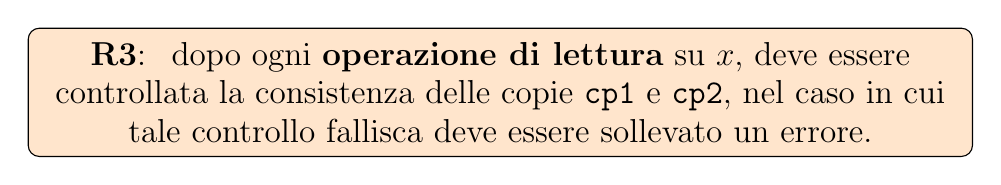
\begin{tikzpicture}
        \node [mybox] (box){%
            \begin{minipage}{.96\textwidth}    
                \begin{center}
                    \large
                    \textbf{R3}:  dopo ogni \textbf{operazione di lettura} su $x$, deve essere controllata la consistenza delle copie \texttt{cp1} e \texttt{cp2}, nel caso in cui tale controllo fallisca deve essere sollevato un errore.
                \end{center}
            \end{minipage}
        };
    \end{tikzpicture}%
\end{center}
Per chiarire l'implementazione della terza regola, si riporta un frammento differente della funzione usata in precedenza: 

\begin{lstlisting}[language=rust, style=boxed]
//uso di assign()
let mut a = Hardened::from(4); 
let mut b = Hardened::from(2); 
a.assign(b);  //'a=b'

pub fn assign(&mut self, other: Hardened<T>)->Result<(), IncoherenceError>{
    //Regola 3: lettura, controllo di coerenza, errori
    if other.incoherent(){
        return Err(IncoherenceError::AssignFail)
    }
    // [...]
}
fn incoherent(&self)->bool{ self.cp1 != self.cp2 }
\end{lstlisting}
Usando la funzione \texttt{assign()}, poiché leggo la variabile \texttt{b} è necessario un controllo di consistenza delle due copie, questo è espletato dalla funzione \texttt{incoherent()} che ritorna un booleano. In caso in cui questo test non viene passato, si ritorna un \texttt{Err(IncoherenceError)}.

\subsection{Gestione degli errori}
La regola \textbf{R3} richiede che, nel caso il controllo di coerenza fallisca, venga sollevato un errore. Si sono utilizzati principalmente due meccanismi per asserire a questo task:
\begin{enumerate}
    \item Propagazione di un errore di tipo \texttt{IncoherenceError} 
    \item \textbf{Uso della macro \texttt{panic!(...)}}
\end{enumerate}
Il motivo per il quale si è avuta la necessità di distinguere questi due casi è legata alle caratteristiche del linguaggio Rust. In particolare, alcuni tratti della libreria standard permettono -- usando la programmazione generica -- di personalizzare sia il tipo dei dati su cui si opera sia il tipo dei valori di ritorno. In altre situazioni, ad esempi nei tratti associati alle \textit{operazioni di confronto}, non è possibile modificare la \textit{firma dei metodi}. Questo è il caso in cui ci si riserva la possibilità di generare un \texttt{panic!(...)} nel caso di anomalia rilevata, lasciando però invariata la firma dei metodi garantendo la correttezza sintattica.
Di seguito si mostrano due esempio in cui si chiariscono meglio gli aspetti appena introdotti:
 

\begin{multicols}{2}
\noindent
\textbf{Uso di \texttt{IncoherenceError} }
\begin{lstlisting}[language=Rust, style=boxed]
impl Add<usize> for Hardened<usize>{
  type Output = Result<Hardened<usize>, 
                    IncoherenceError>;
  fn add(self, rhs: usize) -> Self::Output {
    if self.incoherent() {
        return Err(IncoherenceError::AddFail);
    }
    Ok(Self{
        cp1: self.cp1 + rhs,
        cp2: self.cp2 + rhs,
    })
  }
}
\end{lstlisting}
Si presenta qui l'implementazione del metodo \texttt{add()} del tratto omonimo. La presenza del tipo associato al tratto, permette di non essere vincolati sul tipo di ritorno che quindi è stato personalizzato secondo le nostre esigenze. In particolare poiché l'add come tutte le operazioni di lettura e modifica possono causare errori dovuti all'incoerenza tra le copie interne del dato, si sfrutta l'enumerazione generica \texttt{Result<T,E>} per gestire queste due situazioni. Il tipo \texttt{T} è \texttt{Hardened<T>} mentre il tipo \texttt{E} è quello personalizzato (\texttt{IncoherenceError} descritto in seguito). Un ragionamento analogo vale per tutti i metodi che hanno una struttura simile a quella presentata che abilita l'utilizzo di dati di ritorno personalizzati. 

\newcolumn
\noindent
\textbf{Uso di \texttt{panic!(...)}}
\begin{lstlisting}[language=Rust, style=boxed]
impl<T> Ord for Hardened<T>{
    fn cmp(&self, other: &Self) -> Ordering {
        if other.incoherent(){
            panic!("Ord::cmp");
        }
        self.cp1.cmp(&other.cp1)
    }
}
\end{lstlisting}
Un esempio significativo del caso in cui siamo vincolati  sulla scelta del tipo di ritorno viene presentato. In particolare la funzione \texttt{cmp(...)} del tratto \texttt{Ord} per ovvi motivi vincola il tipo di ritorno ad essere l'enumerativo \texttt{Ordering}. Nel caso in cui il dato letto sia "incoerente", viene sollevato un \texttt{panic!(...)}. Il messaggio è di cruciale importanza per l'invio dei risultati dell'iniettore verso l'analizzatore. \\
\hrule
\vspace{0.5cm}
\noindent
Le due casistiche, come si vedrà, nel \textit{processo di fault injection} vengono gestite in modo diverso, mentre per l'analisi il tipo di informazione associato ai due eventi è analogo.

\end{multicols}

\subsubsection{Il tipo di errore \texttt{IncoherenceError}}
Al fine di personalizzare la semantica degli errori e di facilitare il processo di analisi dei risultati, si è pensato di implementare un \textbf{tipo di errore personalizzato} denominato \texttt{IncoherenceError}. Il crate \textbf{\texttt{thiserror}} permette di derivare l'implementazione del tratto \texttt{Error} richiesta da altri meccanismi interni al linguaggio quali la propagazione tramite \textit{question mark operator} e la descrivibilità dell'errore stesso. Il tipo introdotto è un enumerativo: 

\begin{lstlisting}[language=Rust, style=boxed]
#[derive(Error, Debug, Clone)]
pub enum IncoherenceError{
    #[error("IncoherenceError::AssignFail: assignment failed")]
    AssignFail,
    #[error("IncoherenceError::AddFail: due to incoherence add failed")]
    AddFail,
    #[error("IncoherenceError::MulFail: due to incoherence mul failed")]
    MulFail,
    #[error("IncoherenceError::Generic: generic incoherence error")]
    Generic
}
\end{lstlisting}
Questo costituisce il tipo \texttt{E} integrato nella variante \texttt{Err(E)} di \texttt{Result}. Con quest'ultimo dettaglio si ha il quadro completo delle trasformazioni del codice atte ad introdurre ridondanza nei dati con le operazioni associate e la gestione degli errori. \\
Nella prossima sezione si introducono i casi di studio, questi costituiscono l'applicazione di tutti i concetti che abbiamo visto finora sull'irrobustimento del codice.


\section{Fault List Manager}

\subsection{Analisi statica automatica del codice}

\subsection{Generazione della fault list}

\subsection{Stage pipeline}
\newpage
\section{Injector}\label{sec: Injector}
\subsection{Aspetti Generali}
L'iniettore e' stato pensato come un componente della pipeline che riceve le fault list entry dal fault list manager, utilizzandole poi per iniettare gli errori nel momento 
corretto durante l'esecuzione dell'algoritmo tesato. Il risultato dell'esecuzione viene poi utilizzato per creare il TestResult relativo alla singola fault list entry e passato 
al successivo stadio della pipeline. 

Per l'implementazione dell'iniettore vengono utilizzati 2 thread, uno per l'esecuzione dell'algoritmo che chiameremo \textit{runner}, e uno per l'esecuzione dell'i\-niettore che 
chiameremo \textit{injector}. I due thread condividono le variabili in uso che, durante un'istanza dell'esecuzione dell'algoritmo sotto esame (un'istanza per ciascuna fault list 
entry), verranno lette e modificate da entrambi i thread: il thread runner leggera' e modifichera' le variabili seguendo l'ordine delle istruzioni dell'algoritmo, il thread
injector leggera' la variabile su cui iniettare l'errore per poter calcolare il nuovo valore (ovvero quello contenente l'errore) e modificandola di conseguenza. Affinche' i due 
thread si sincronizzino correttamente e l'iniezione dell'errore avvenga nell'istante specificato nella fault list entry, i due thread utilizzano 2 canali monodirezionali \textit{mpsc} in modo che 
dopo ogni istruzione dell'algoritmo eseguita dal runner venga mandato un messaggio all'injector su un canale e ne venga attesa la risposta sull'altro. L'\textit{injector}

\subsection{Aspetti tecnici}
\subsubsection{Injector Manager}
La funzione chiamata \textit{injector\_manager} ha la funzione di coordinare la ricezione delle fault list entry provenienti dallo stato precedente della pipeline tramite un canale dedicato, ricevendo anche il canale per trasmettere i risultati, l'algoritmo target e i dati da usare durante l'analisi.

\begin{lstlisting}[language=Rust, style=boxed]
pub fn injector_manager(rx_chan_fm_inj: Receiver<FaultListEntry>,
                tx_chan_inj_anl: Sender<TestResult>,
                target: String,
                data: Data<i32>);
\end{lstlisting}

Al suo interno la funzione tramite un ciclo while attende la ricezione sul canale delle fault list entry e, per ciascuna, crea il set di variabili utilizzate (in base al tipo di algoritmo in esecuzione), i 2 canali con cui i thread gestiranno la sincronizzazione e i 2 thread \textit{runner} e \textit{injector}.

Affinche' siano testabili piu' algoritmi, ciascuno avente il proprio set di variabili che utilizza, e' stata usata un'enum chiamata \textit{AlgorithmVariables} contenente per ciascun algoritmo una struct contenente le variabili.

\begin{lstlisting}[language=Rust, style=boxed]
enum AlgorithmVariables {
    SelectionSort(SelectionSortVariables),
    BubbleSort(BubbleSortVariables),
    MatrixMultiplication(MatrixMultiplicationVariables),
}
\end{lstlisting}

Le struct relative ai singoli algoritmi contengono, per ogni variabile, un \textit{RwLock} contenente a sua volta il tipo \textit{Hardened} corrispondente. Dovendo condividere questa struttura tra piu' thread eseguiti, era necessario renderla accessibile in modo sicuro (dovendo essere sia letta che scritta) e per questo motivo una possibile soluzione era quella di racchiudere la struttura per intero all'interno di un \textit{Mutex} o \textit{RwLock}. Questa soluzione presentava pero' delle criticita'. Per effettuare il controllo condizionale per i cicli while era richiesto di acquisire il lock prima del check sulla condizione del ciclo, ma una volta acquisito il lock fuori dal ciclo questo veniva mantenuto per l'intera durata del ciclo, impedendo all'\textit{injector} di iniettare l'errore su una delle variabili. Di conseguenza l'opzione migliore e che richiedesse meno overhead a livello di codice era racchiudere ciascuna singola variabile della struct in un RwLock anziche' la struttura per intero. La scelta di utilizzare RwLock e' stata motivata principalmente da una possibile migliore gestione delle read e write, dovuta a numero di letture e scrittura sbilanciato in base all'algoritmo eseguito.

\begin{lstlisting}[language=Rust, style=boxed]
struct SelectionSortVariables {
    i: RwLock<Hardened<usize>>,
    j: RwLock<Hardened<usize>>,
    N: RwLock<Hardened<usize>>,
    min: RwLock<Hardened<usize>>,
    vec: RwLock<Vec<Hardened<i32>>>,
}
\end{lstlisting}

Una volta creata la struct contenente le variabili della fault list entry corrente, vengono aperti i canali di comunicazione tra \textit{runner} e \textit{injector} ed eseguiti i rispettivi due thread. Quando il thread \textit{runner} termina invia all'analizzatore (stadio di pipeline successivo) i risultati ottenuti.

\subsubsection{Runner}
Il thread \textit{runner} esegue una funzione wrapper chiamata \textit{runner} la quale si occupa di lanciare l'esecuzione dell'algoritmo irrobustito corretto per il tipo di analisi che si sta facendo e gestendo il risultato prodotto da questo. 

\begin{lstlisting}[language=Rust, style=boxed]
fn runner(variables: Arc<AlgorithmVariables>,
          fault_list_entry: FaultListEntry,
          tx_runner: Sender<&str>,
          rx_runner: Receiver<&str>) -> TestResult
\end{lstlisting}

In base al tipo di algoritmo \textit{target} sono stati creati degli algoritmi ad-hoc per poter interagire correttamente con l'iniettore. Questi sono delle versioni rivisitate delle versioni irrobustite originali, le quali non sarebbero state in grado di sincronizzarsi con l'iniettore per subire i fault. Di seguito viene descritta la struttura di questi algoritmi, facendo esempi relativi al Selection Sort, in quanto gli altri seguono tutti la stessa logica. 

\paragraph{Algoritmo Testato}
Ciascun algoritmo riceve le variabili da utilizzare, il canale su cui trasmettere il completamento di un'istruzione e quello su cui attendere l'eventuale inserimento del fault.

\begin{lstlisting}[language=Rust, style=boxed]
pub fn runner_matrix_multiplication(variables: &MatrixMultiplicationVariables, 
            tx_runner: Sender<&str>, 
            rx_runner: Receiver<&str>) -> Result<(), IncoherenceError>
\end{lstlisting}

La procedura per l'esecuzione di una qualsiasi istruzione e':
\begin{itemize}
    \item Accesso al lock con conseguente lettura/scrittura della variabile
    \item Scrittura sul canale \textit{tx\_runner} per comunicare all'\textit{injector} che un'istruzione e' stata eseguita
    \item Attesa sul canale \textit{rx\_runner} che l'\textit{injector} termini le sue operazioni, necessario affinche' \textit{runner} e \textit{injector} rimangano sincronizzati
\end{itemize}

Riportiamo di seguito un esempio di un'istruzione equivalente all'istruzione $j.assign((i+1)?)?$:
\begin{lstlisting}[language=Rust, style=boxed]
// j = i + 1   -- versione non irrobustita
// j.assign((i+1)?)?    -- versione irrobustita
variables.j.write().unwrap().assign((*variables.i.read().unwrap() + 1)?)?;
tx_runner.send("").unwrap();
rx_runner.recv().unwrap();
\end{lstlisting}

L'algoritmo ritorna un Result, contenente:
\begin{itemize}
    \item \textit{Ok(())}: successo ed esecuzione portata a termine correttamente'
    \item \textit{Err$<$IncoherenceError$>$}: variante dell'enum \textit{IncoherenceError} che descrive il tipo di errore riscontrato 
\end{itemize}

\paragraph{Terminazione Runner}
Il runner termina eseguendo un pattern match sul risultato dell'algoritmo eseguito, producendo il TestResult che verra' utilizzato dall'analizzatore per ottenere statistiche utili.

\subsection{Injector}
L'\textit{injector} e' una funzione che si occupa di iniettare nel momento corretto il fault contenuto nella fault list entry sulla variabile indicata. Per fare cio', riceve le variabili usate dall'algoritmo e condivise con il \textit{runner}, la fault list entry e i canali necessari per la sincronizzazione con il \textit{runner}.

\begin{lstlisting}[language=Rust, style=boxed]
fn injector(variables: Arc<AlgorithmVariables>, 
            fault_list_entry: FaultListEntry,
            tx_injector: Sender<&str>,
            rx_runner: Receiver<&str>)
\end{lstlisting}

L'informazione sul tipo di algoritmo in esecuzione e' ricavata dal tipo di variabili ricevute, essendo queste un'istanza dell'enum \textit{AlgorithmVariables}. Viene poi manutenuto un \textit{counter} necessario a contare il numero di istruzioni eseguite per poi al momento indicato nella fault list entry iniettare l'errore. Tramite un ciclo while, che termina quando il canale condiviso con il \textit{runner} viene chiuso, vengono ricevuti gli impulsi che indicano la terminazione di un'istruzione. Il flusso di operazioni eseguite e': 

\begin{enumerate}
    \item Calcola la maschera in base al bit indicato nella fault list entry
    \item Per ogni segnale ricevuto dal \textit{runner}:
    \begin{enumerate}
        \item Incrementa il counter
        \item Se $\textit{counter} == \textit{fault\_list\_entry}.\textit{time}$
        \begin{enumerate}
            \item Ricava la variabile su cui iniettare contenuta nella fault list entry
            \item Tramite match inietta sulla variabile la maschera calcolata
        \end{enumerate}
        \item Manda sul canale verso il \textit{runner} il segnale per la continuazione della sua esecuzione
    \end{enumerate}
\end{enumerate}

Le maschere vengono calcolate come $\textit{mask} = 2^{\textit{fault\_mask}}$. Le maschere vengono applicate alle variabili tramite XOR. Prendendo un esempio per quanto riguarda il Selection Sort:
\begin{lstlisting}[language=Rust, style=boxed]
"i" => {
    let val = var.i.read().unwrap().inner().unwrap().clone();   // leggo il valore della variabile
    let new_val = val \wedge mask;                                   // nuovo valore da salvare (XOR per il bitflip)
    var.i.write().unwrap()["cp1"] = new_val;                    // inietto l'errore
}
\end{lstlisting}

















\section{Analizzatore}\label{sec:analizer}
\section{Casi di studio}

\subsection{Selection Sort}

\subsection{Bubble Sort}

\subsection{Moltiplicazioni tra matrici}

\printbibliography


\end{document}
